\section{Наблюдатель пониженного порядка}
Рассмотрим систему:
\begin{equation}
    \begin{array}{ll}
        \dot{x} = Ax + Bu\\
        y = Cx + Du
    \end{array}
\end{equation}
где
\begin{equation}
    \begin{array}{cccc}
        A = \begin{bmatrix}
            6 & 0 & -12 & 6 \\ 
            0 & 6 & -6 & 12 \\
            -12 & -6 & 6 & 0 \\
            6 & 12 & 0 & 6
        \end{bmatrix}, & 
        B = \begin{bmatrix}
            6 \\ 12 \\ 6 \\ 4
        \end{bmatrix}, & 
        C = \begin{bmatrix}
            0 & 0 & 1 & 0 \\ 
            0 & 0 & 0 & 1
        \end{bmatrix}, 
        D = \begin{bmatrix}
            2 \\ 2
        \end{bmatrix}
    \end{array}
\end{equation}
В вещественной Жордановой форме имеем матрицы:
\begin{equation}
    \begin{array}{cccc}
        A_j = \begin{bmatrix}
            0.00  & 0.00  & 0.00  & 0.00 \\ 
            0.00  & 12.00  & 0.00  & 0.00 \\ 
            0.00  & 0.00  & -12.00  & 0.00 \\ 
            0.00  & 0.00  & 0.00  & 24.00 \\ 
            \end{bmatrix}, &
        P = \begin{bmatrix}
            1.00  & -1.00  & -1.00  & 1.00 \\ 
            -1.00  & 1.00  & -1.00  & 1.00 \\ 
            1.00  & 1.00  & -1.00  & -1.00 \\ 
            1.00  & 1.00  & 1.00  & 1.00 \\ 
            \end{bmatrix}, \\
        B_j = \begin{bmatrix}
            1.00 \\ 
            4.00 \\ 
            -5.00 \\ 
            4.00 \\ 
            \end{bmatrix}, &
        C_j = \begin{bmatrix}
            1.00  & 1.00  & -1.00  & -1.00 \\ 
            1.00  & 1.00  & 1.00  & 1.00 \\ 
            \end{bmatrix}   
    \end{array}
\end{equation}
Можно сделать вывод, что система является полностью управляемой и полностью наблюдаемой.

\subsection{Наблюдатель пониженного порядка}
Рассмотрим наблюдатель пониженного порядка:
\begin{equation}
    \begin{array}{ll}
        \dot{\hat{z}} = \Gamma\hat{z} - Yy + (QB + YD)u\\
        \hat{x} = \begin{bmatrix}
            C \\ Q
        \end{bmatrix}^{-1} \times \begin{bmatrix}
            y - Du \\ 
            \hat{z}
        \end{bmatrix}
    \end{array}
\end{equation}
В качестве регулятора $u = K\hat{x}$ будем использовать регулятор, полученный в предыдущем задании:
\begin{equation}
    K = \begin{bmatrix}
        -3.72  & -2.13  & 3.79  & -2.21 \\ 
    \end{bmatrix}
\end{equation}

Зададим желаемый спектр наблюдателя пониженного порядка $\{-1, -2\}$.

Тогда матрица $Q$ находится из решения уравнения Сильвестра: 
\begin{equation}
   \Gamma Q - QA = YC 
\end{equation}
где $\Gamma$ -- матрица с желаемыми собственными числами. 

Получаем матрицу $Q$:
\begin{eqnarray}
    Q = \begin{bmatrix}
        -0.46  & 0.46  & -0.54  & -0.54 \\ 
        -0.21  & 0.21  & -0.29  & -0.29 \\ 
    \end{bmatrix}
\end{eqnarray}

\subsection{Моделирование}
Схема моделирования представлена на рисунке~\ref{fig:task4_sim}.
\begin{figure}[ht!]
    \centering
    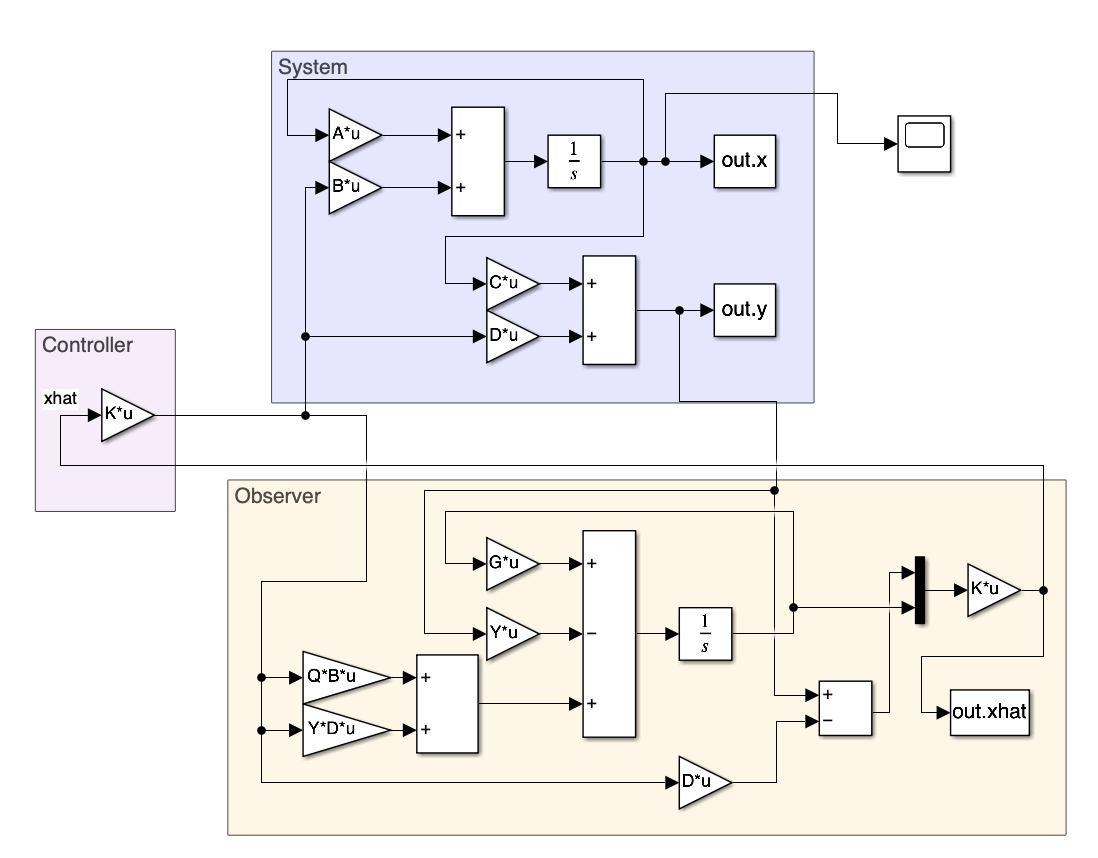
\includegraphics[width=\textwidth]{media/scheme4.png}
    \caption{Схема моделирования наблюдателя пониженного порядка}
    \label{fig:task4_sim}
\end{figure}

Проведем моделирование системы с начальными условиями $x(0) = \begin{bmatrix} 1 & 1 & 1 & 1 \end{bmatrix}^T$ и $\hat{z}(0) = \begin{bmatrix} 0 & 0 \end{bmatrix}^T$.

Результаты моделирования представлены на рисунках \ref{fig:task4_x1_1}, \ref{fig:task4_x2_1}, \ref{fig:task4_x3_1}, \ref{fig:task4_x4_1} (состояния системы), \ref{fig:task4_diff_1} (ошибка наблюдателя), 
рис. \ref{fig:task4_u_1} (управляющее воздействие) и рис. \ref{fig:task4_zhat_1} (вектор состояния наблюдателя $\hat{z}$).

\begin{figure}
    \centering
    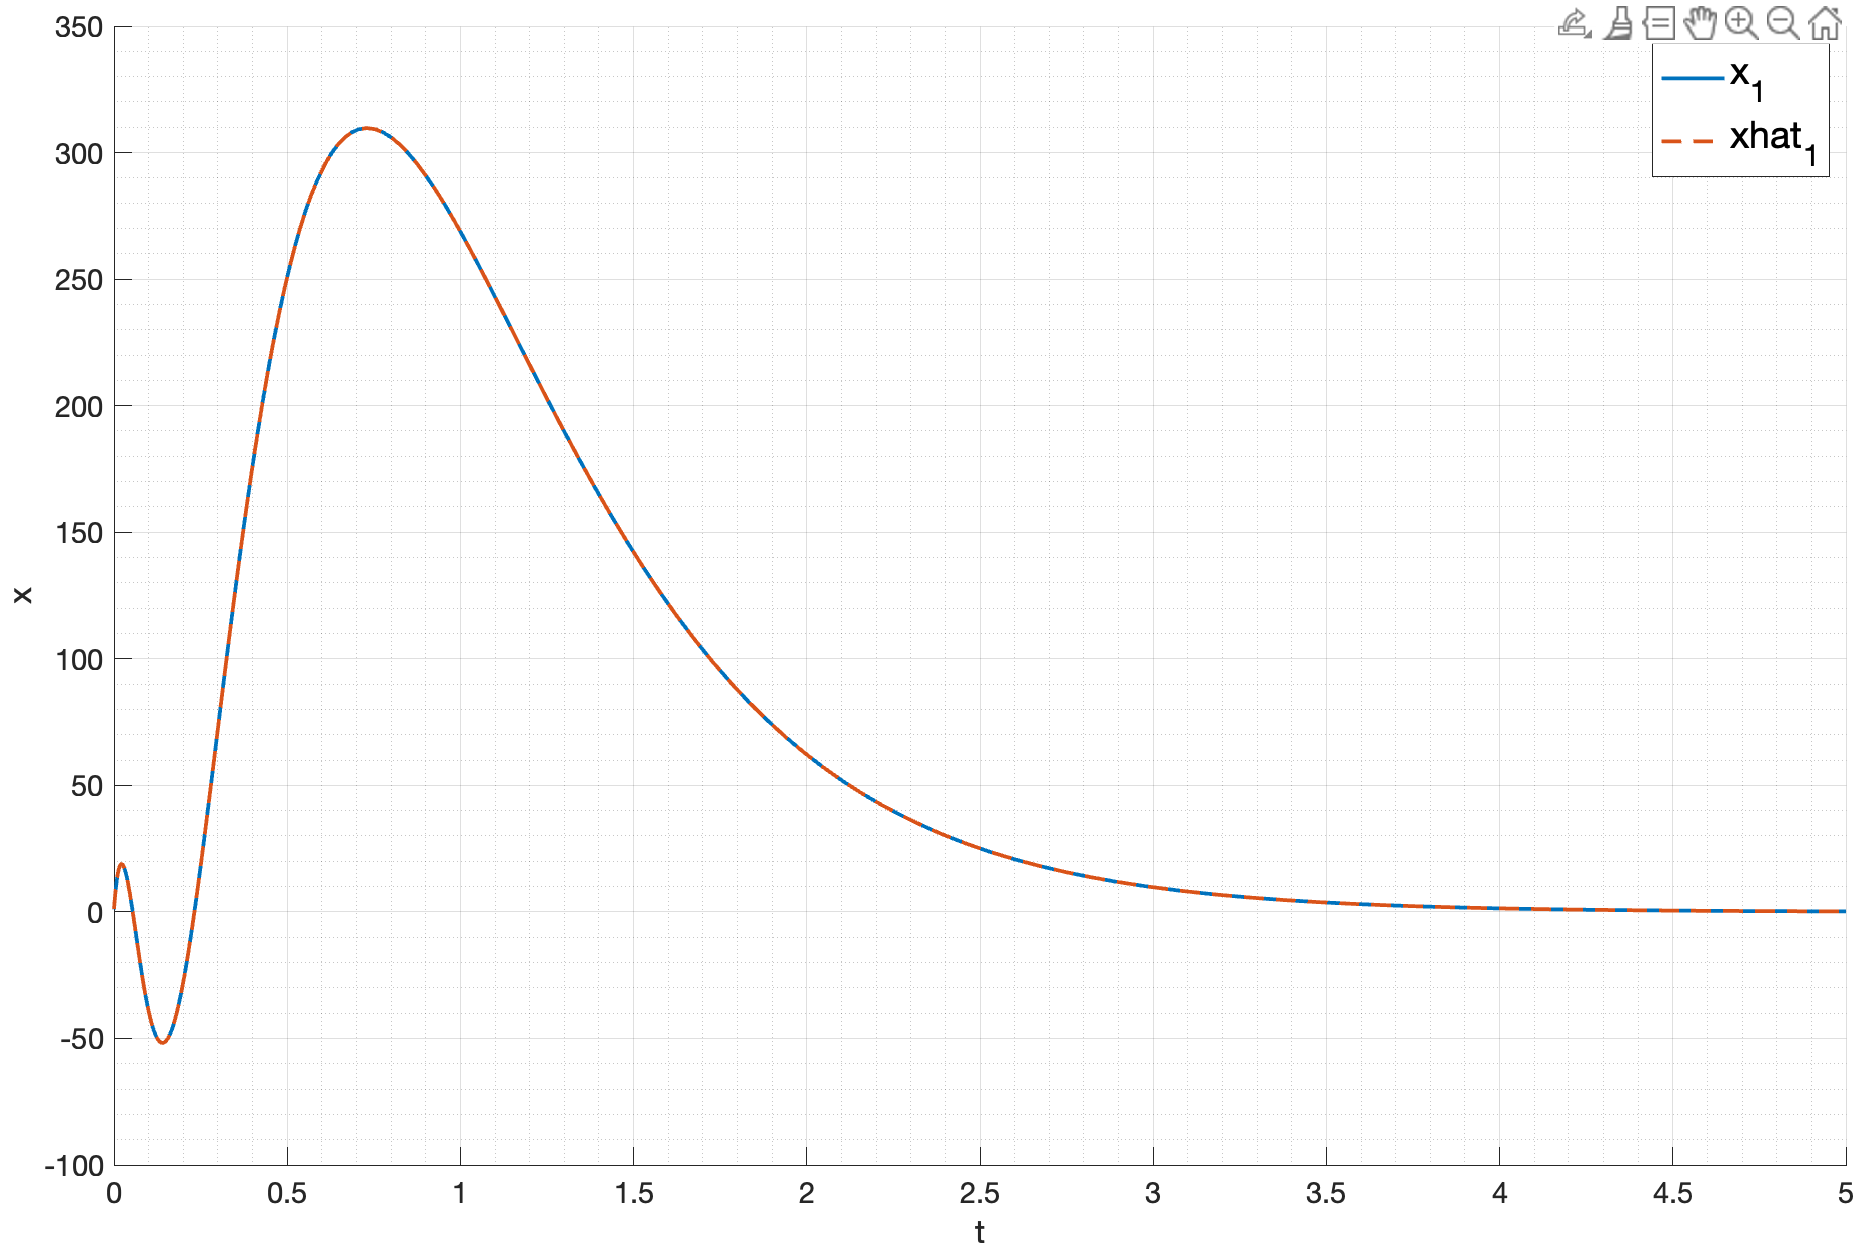
\includegraphics[width=\textwidth]{media/plots/task4_x1_1.png}
    \caption{Состояние системы $x_1$ с наблюдателем пониженного порядка}
    \label{fig:task4_x1_1}
\end{figure}

\begin{figure}
    \centering
    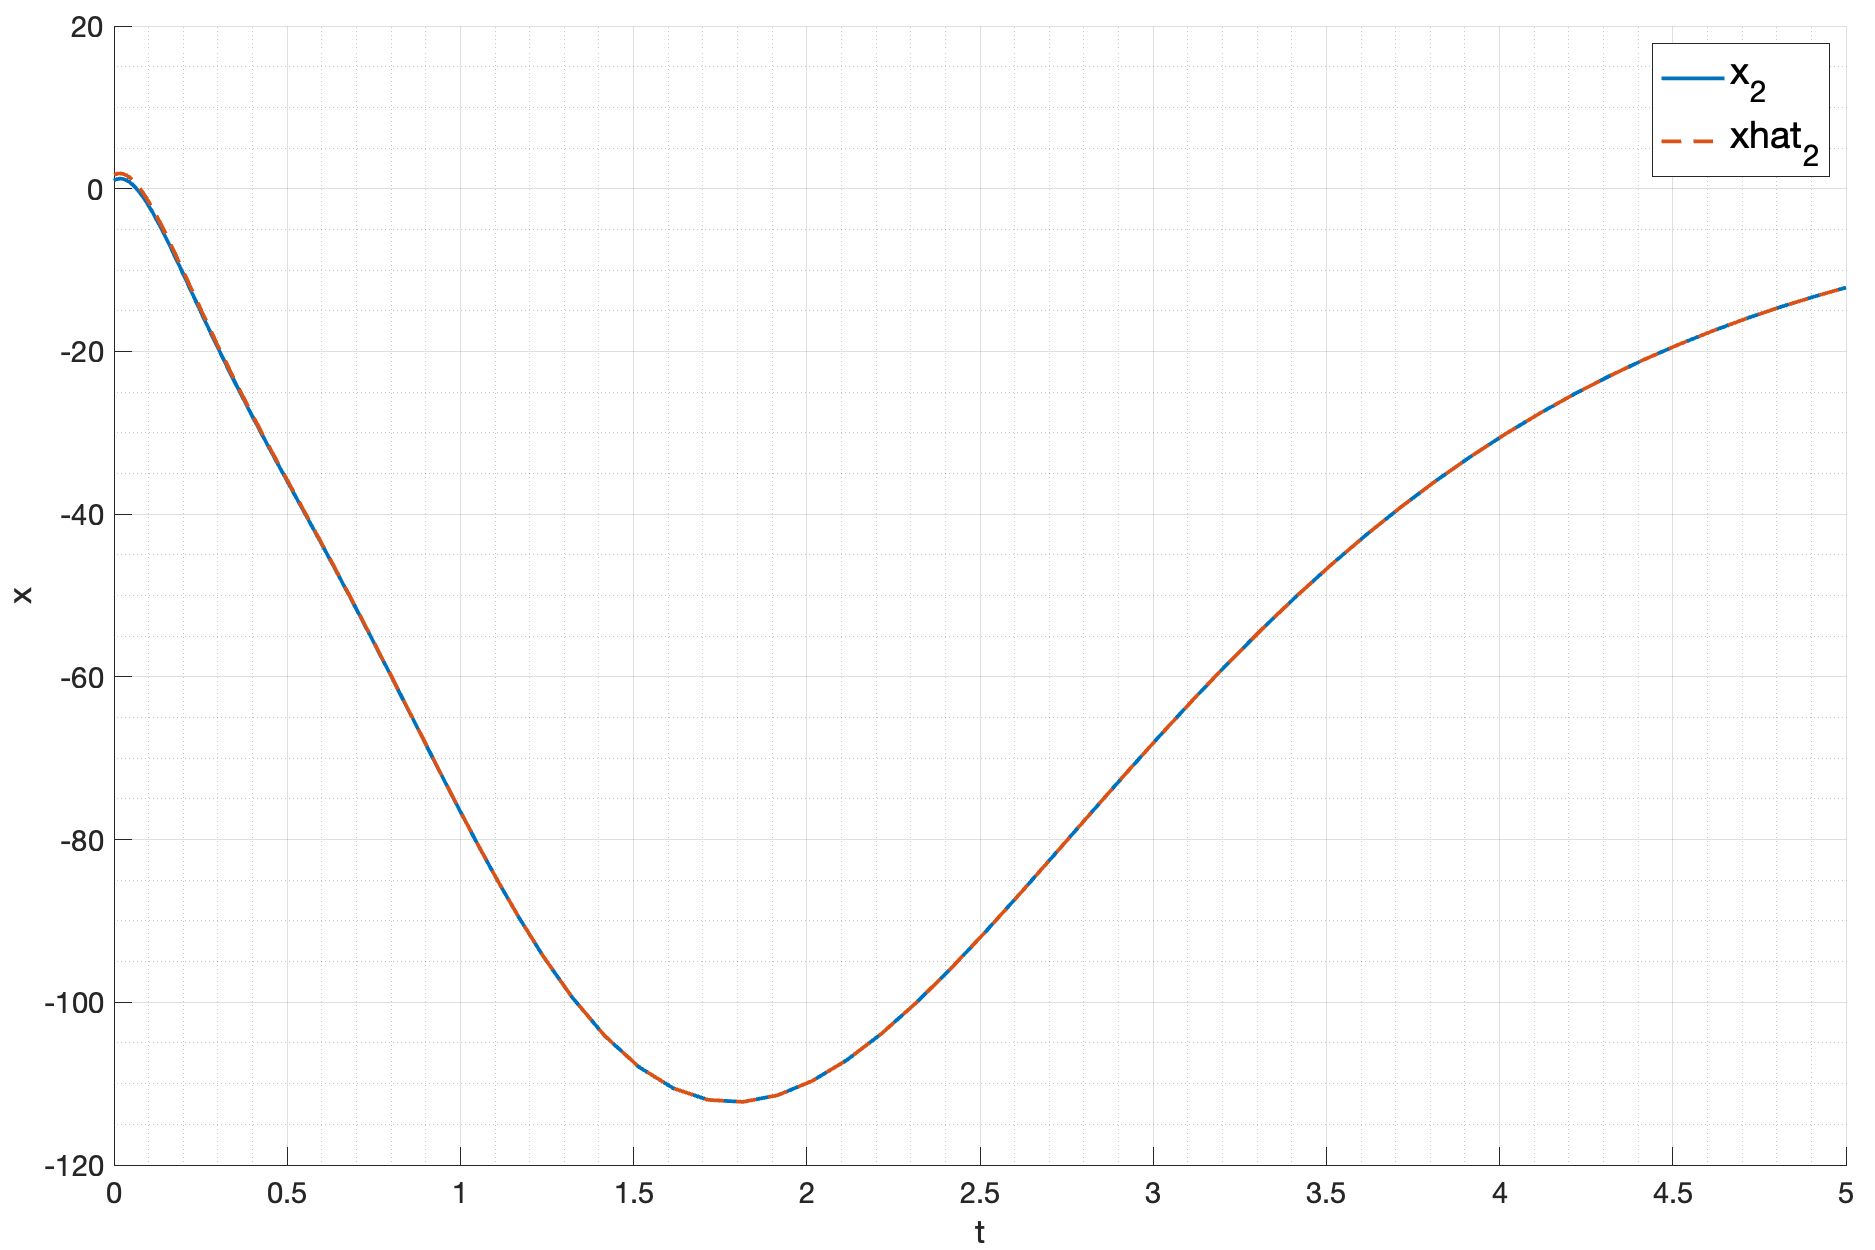
\includegraphics[width=\textwidth]{media/plots/task4_x2_1.png}
    \caption{Состояние системы $x_2$ с наблюдателем пониженного порядка}
    \label{fig:task4_x2_1}
\end{figure}

\begin{figure}
    \centering
    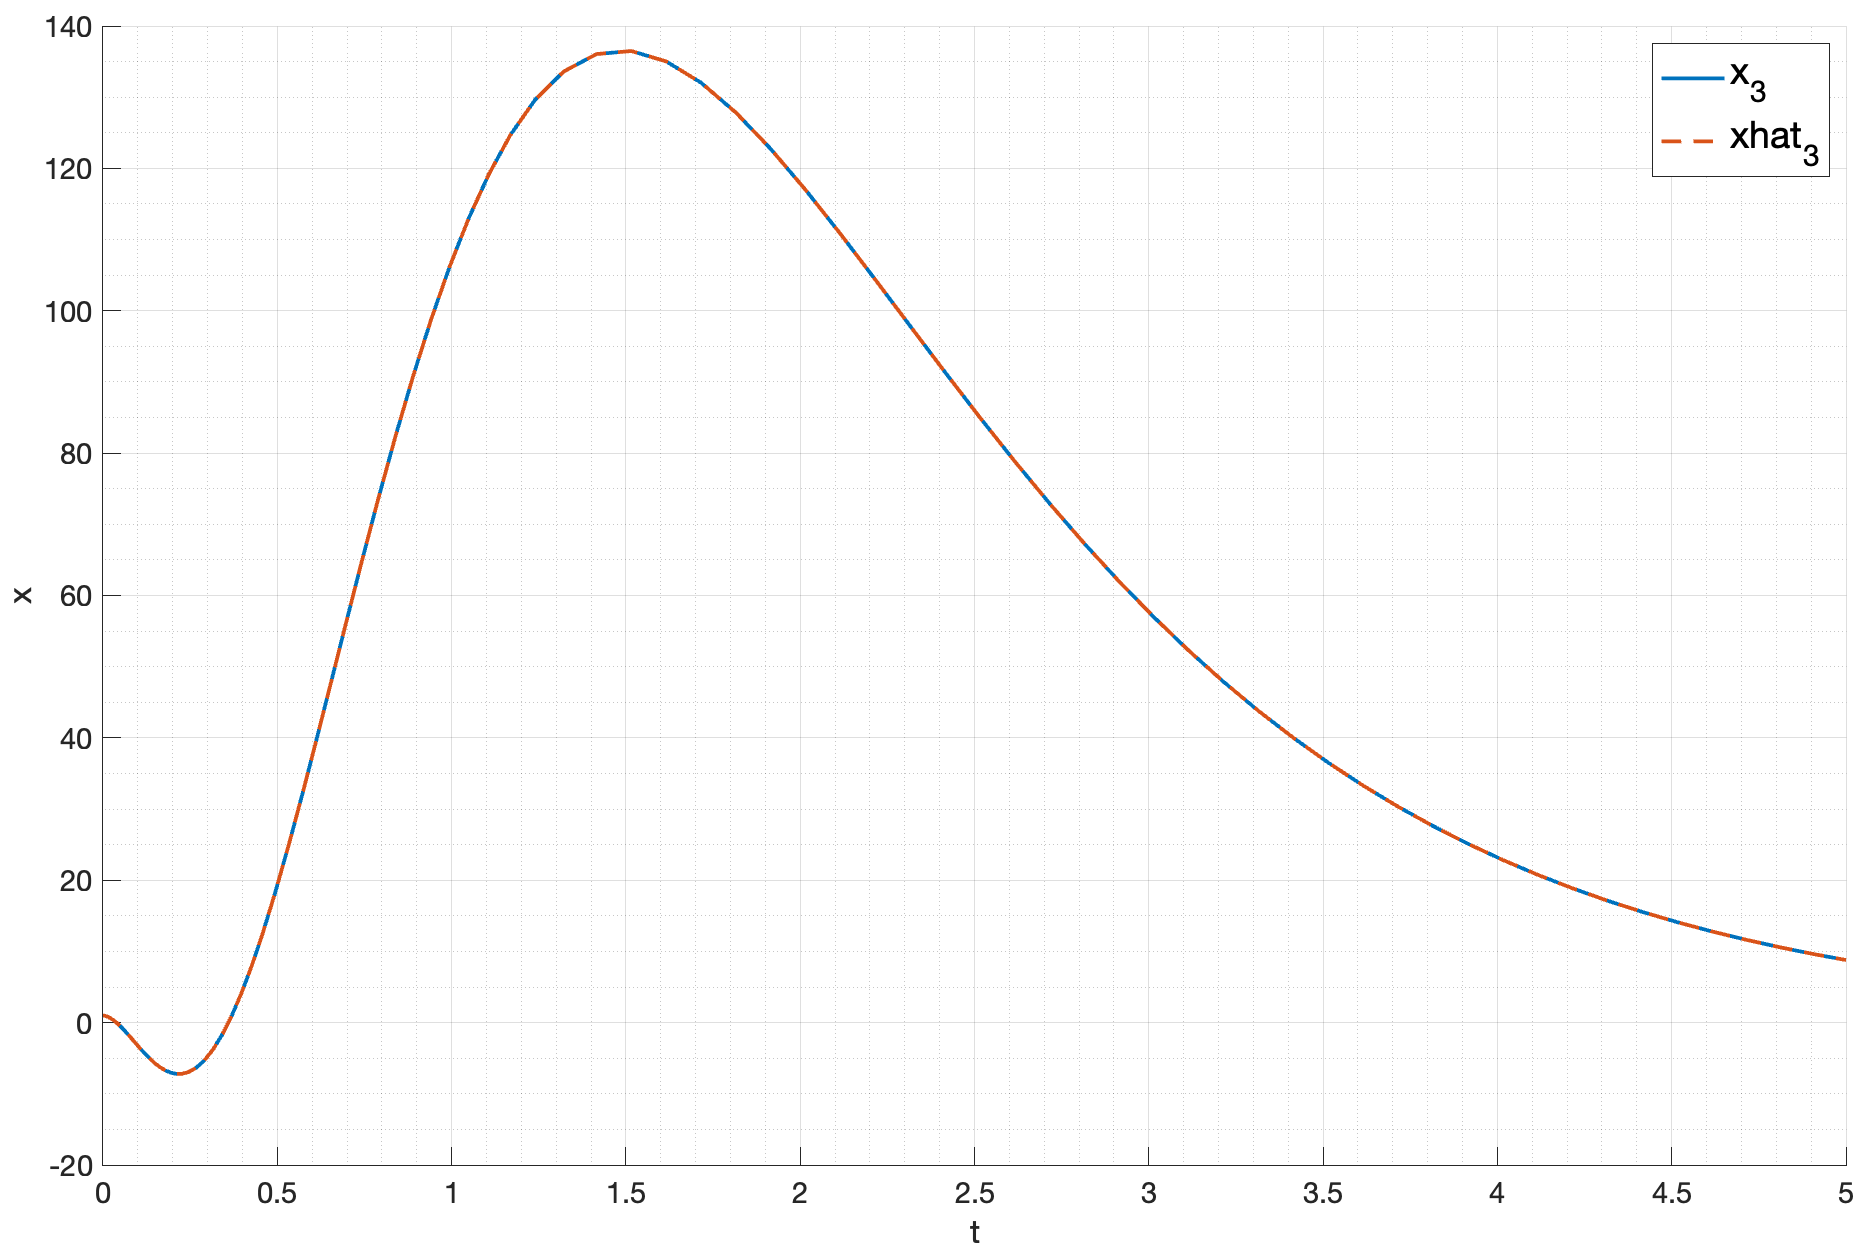
\includegraphics[width=\textwidth]{media/plots/task4_x3_1.png}
    \caption{Состояние системы $x_3$ с наблюдателем пониженного порядка}
    \label{fig:task4_x3_1}
\end{figure}

\begin{figure}
    \centering
    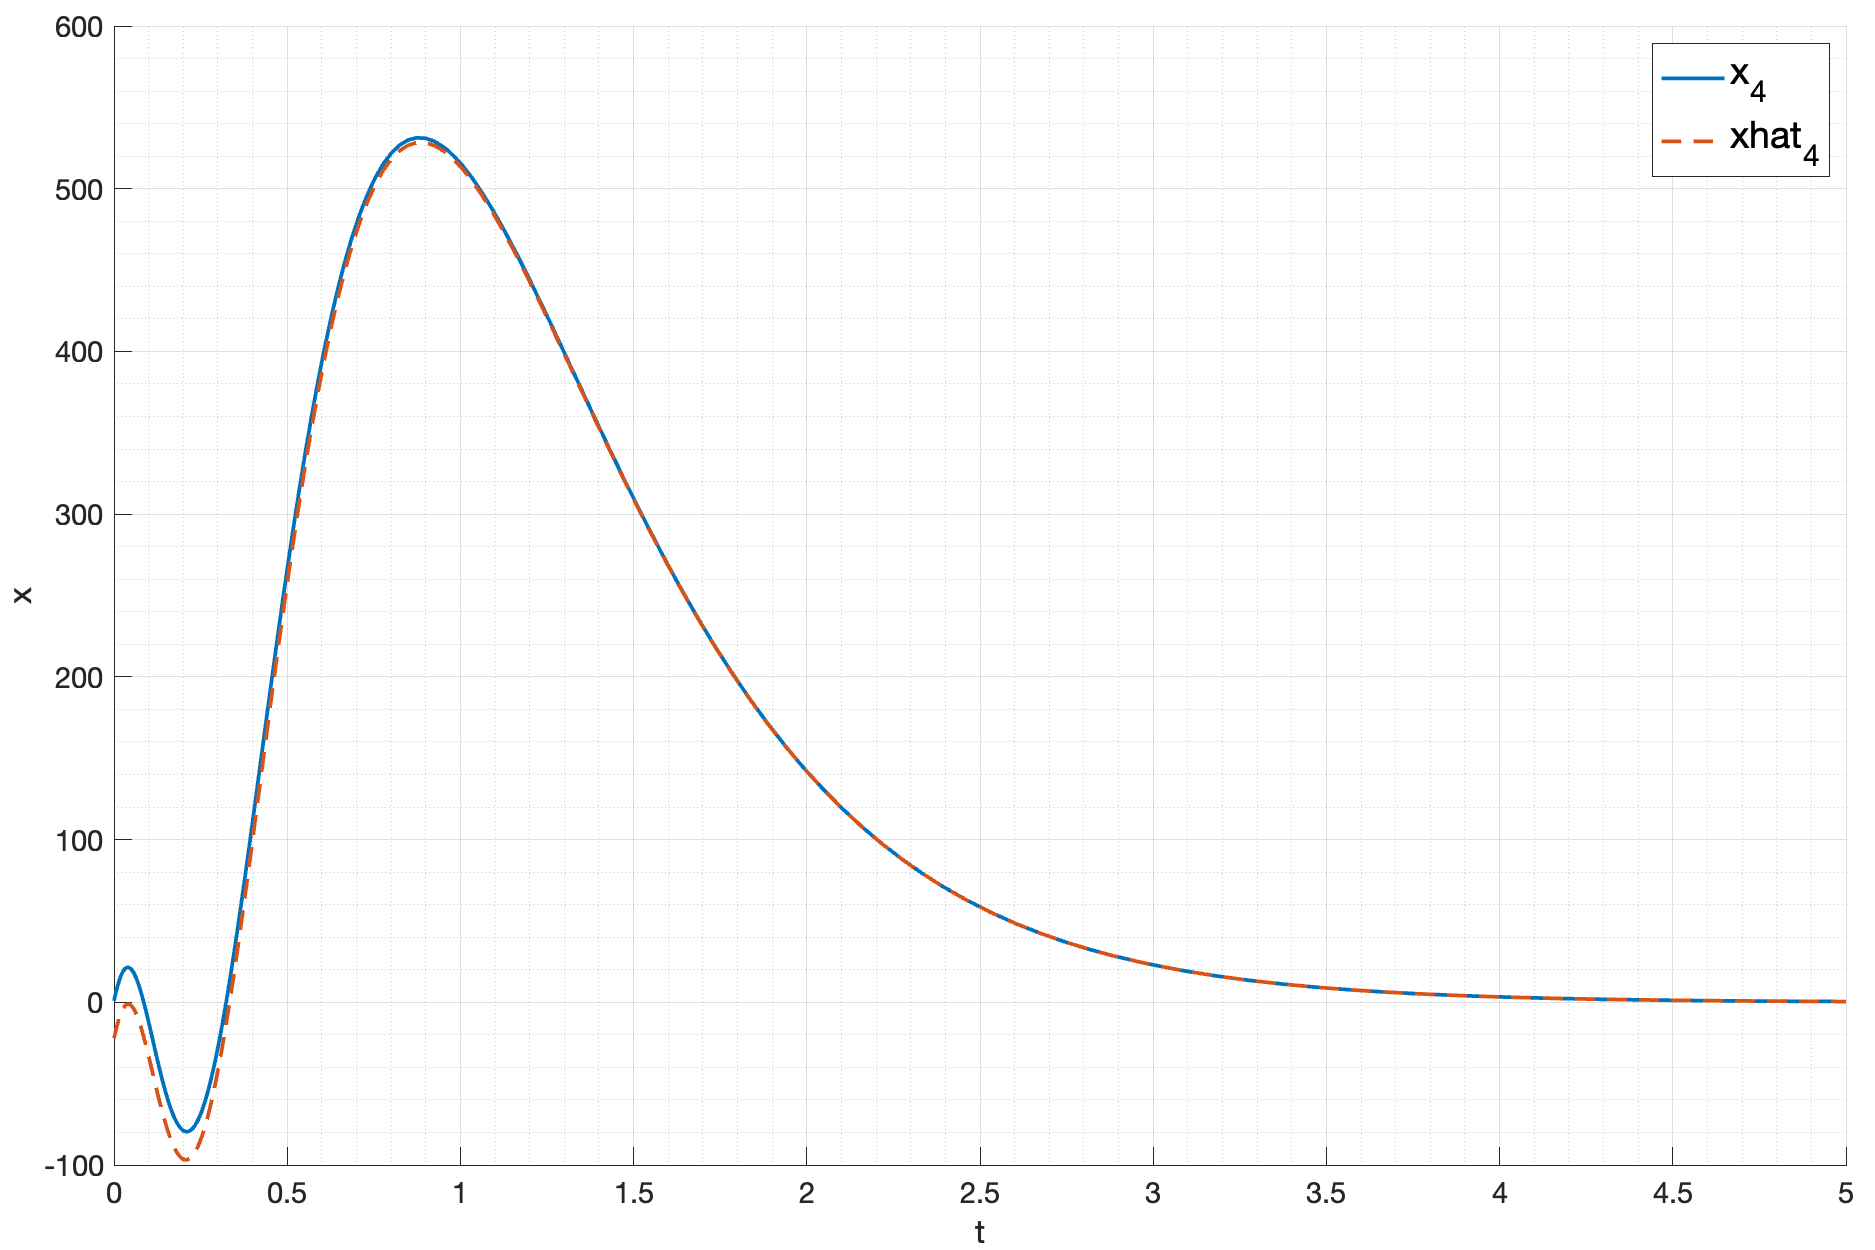
\includegraphics[width=\textwidth]{media/plots/task4_x4_1.png}
    \caption{Состояние системы $x_4$ с наблюдателем пониженного порядка}
    \label{fig:task4_x4_1}
\end{figure}

\begin{figure}
    \centering
    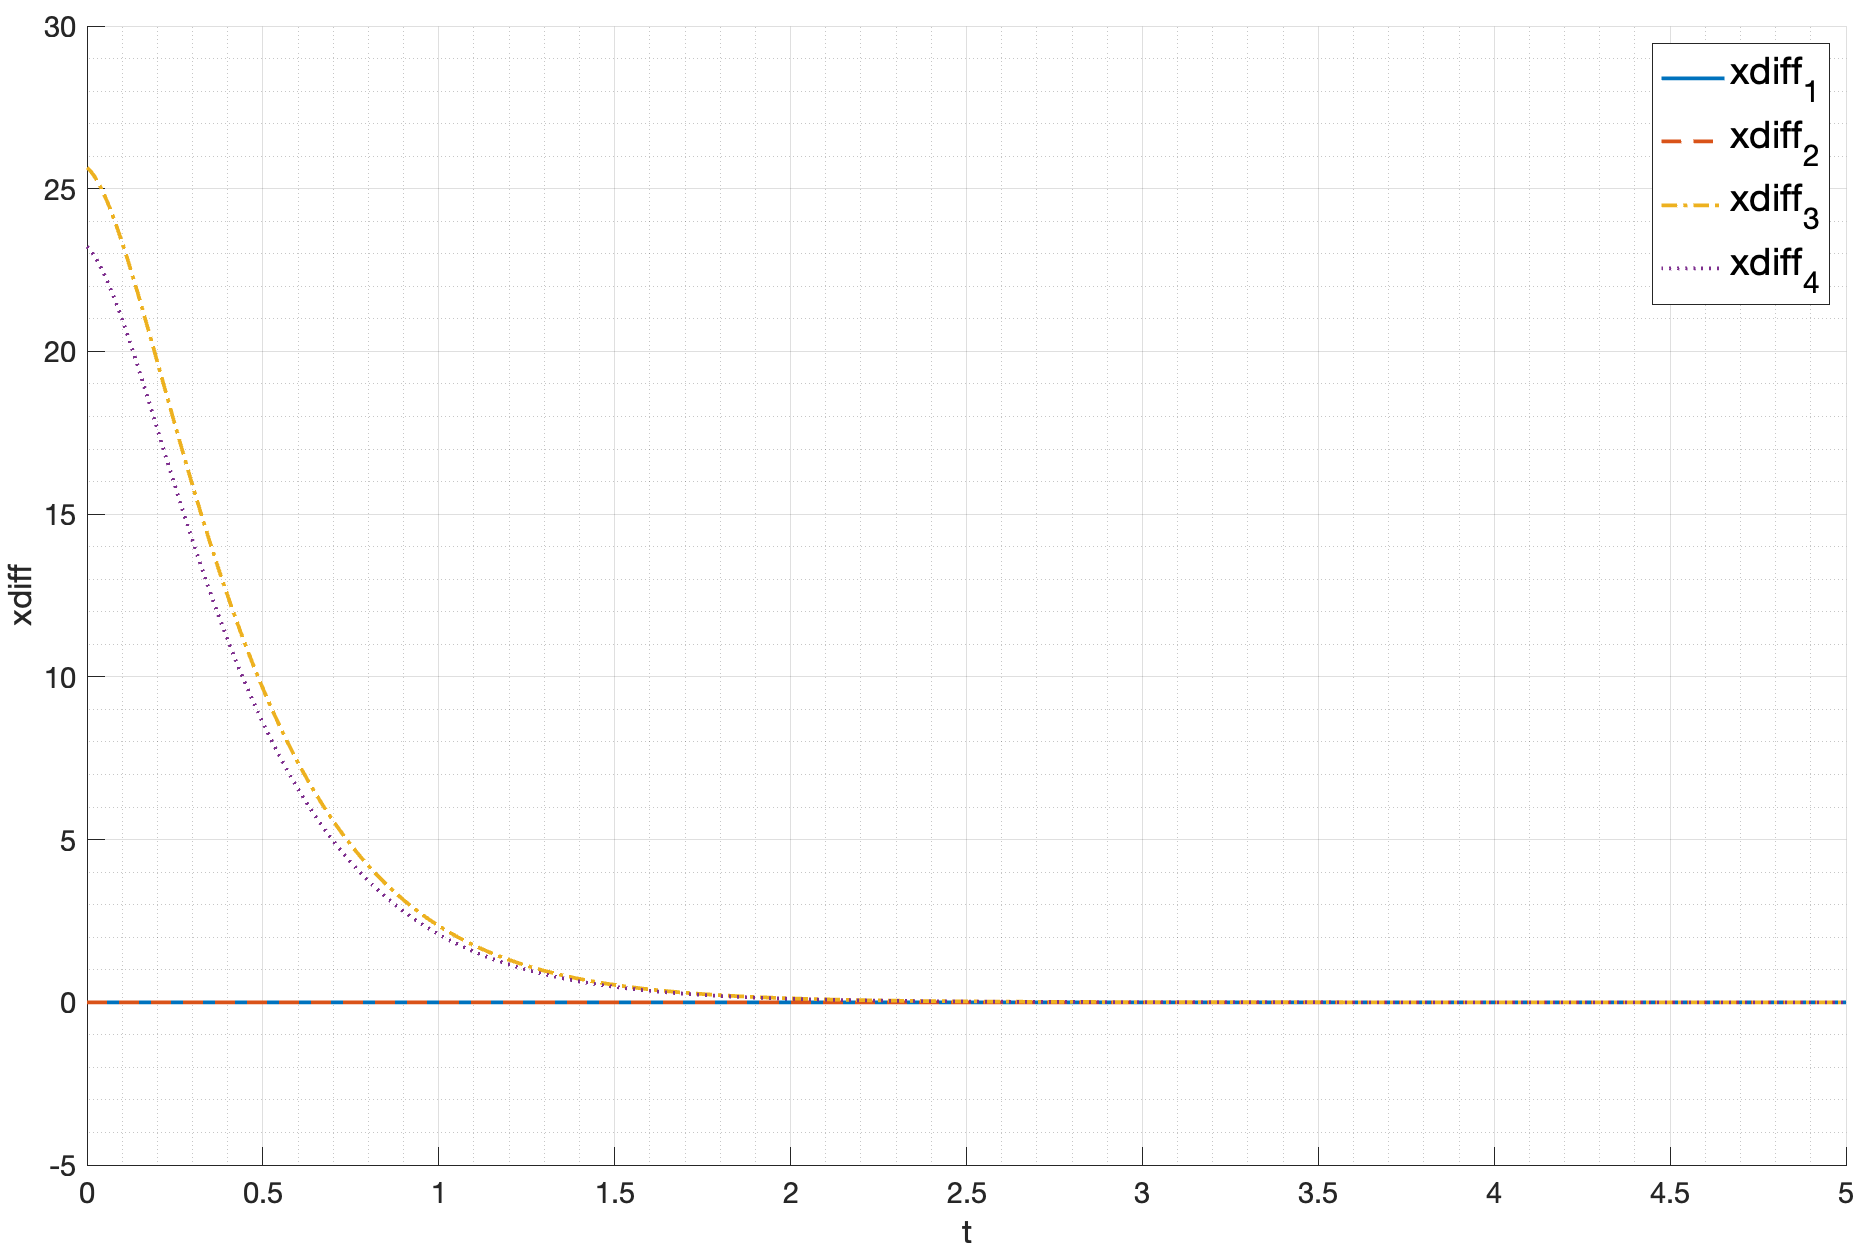
\includegraphics[width=\textwidth]{media/plots/task4_xdiff_1.png}
    \caption{Ошибка наблюдателя пониженного порядка}
    \label{fig:task4_diff_1}
\end{figure}

\begin{figure}
    \centering
    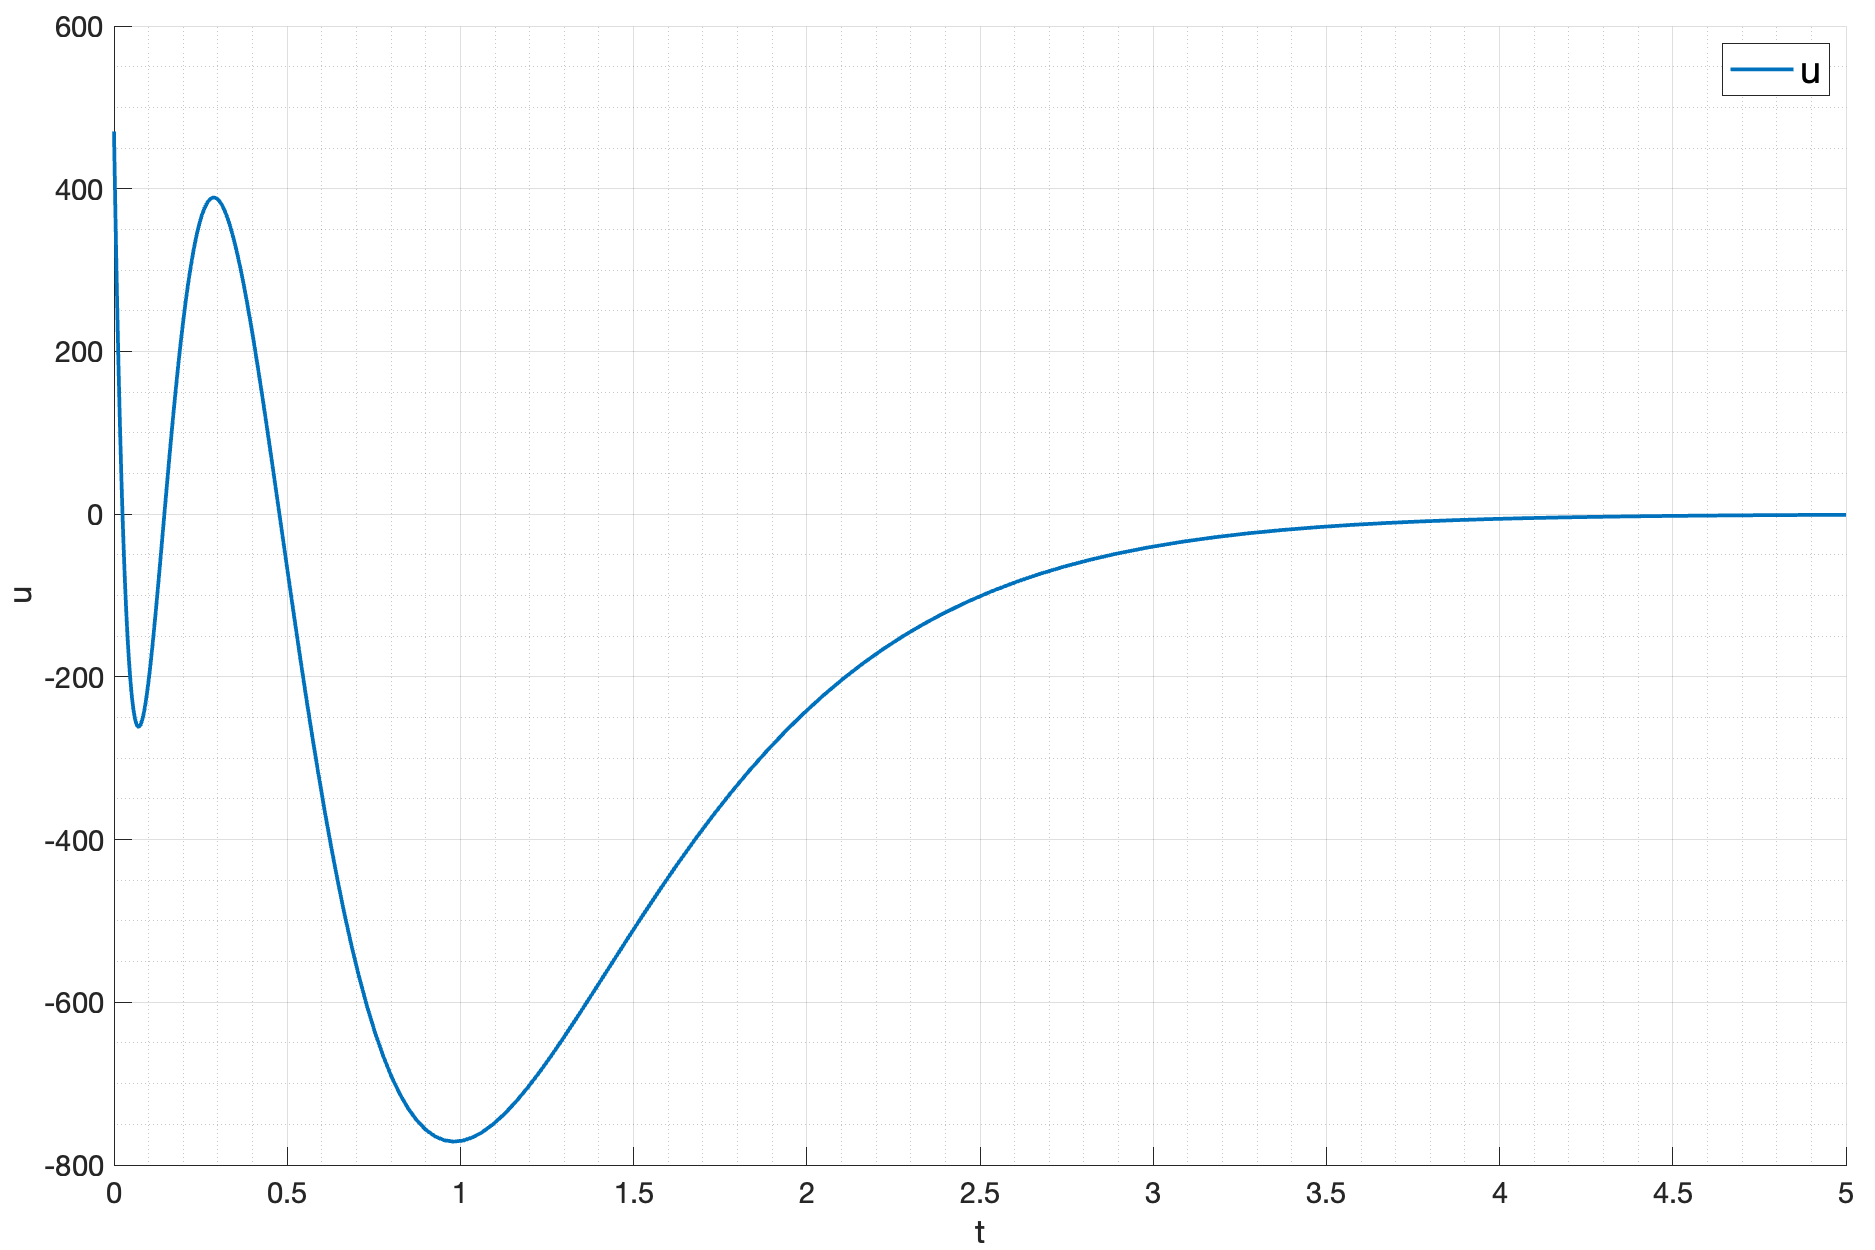
\includegraphics[width=\textwidth]{media/plots/task4_u_1.png}
    \caption{Управляющее воздействие}
    \label{fig:task4_u_1}
\end{figure}

\begin{figure}
    \centering
    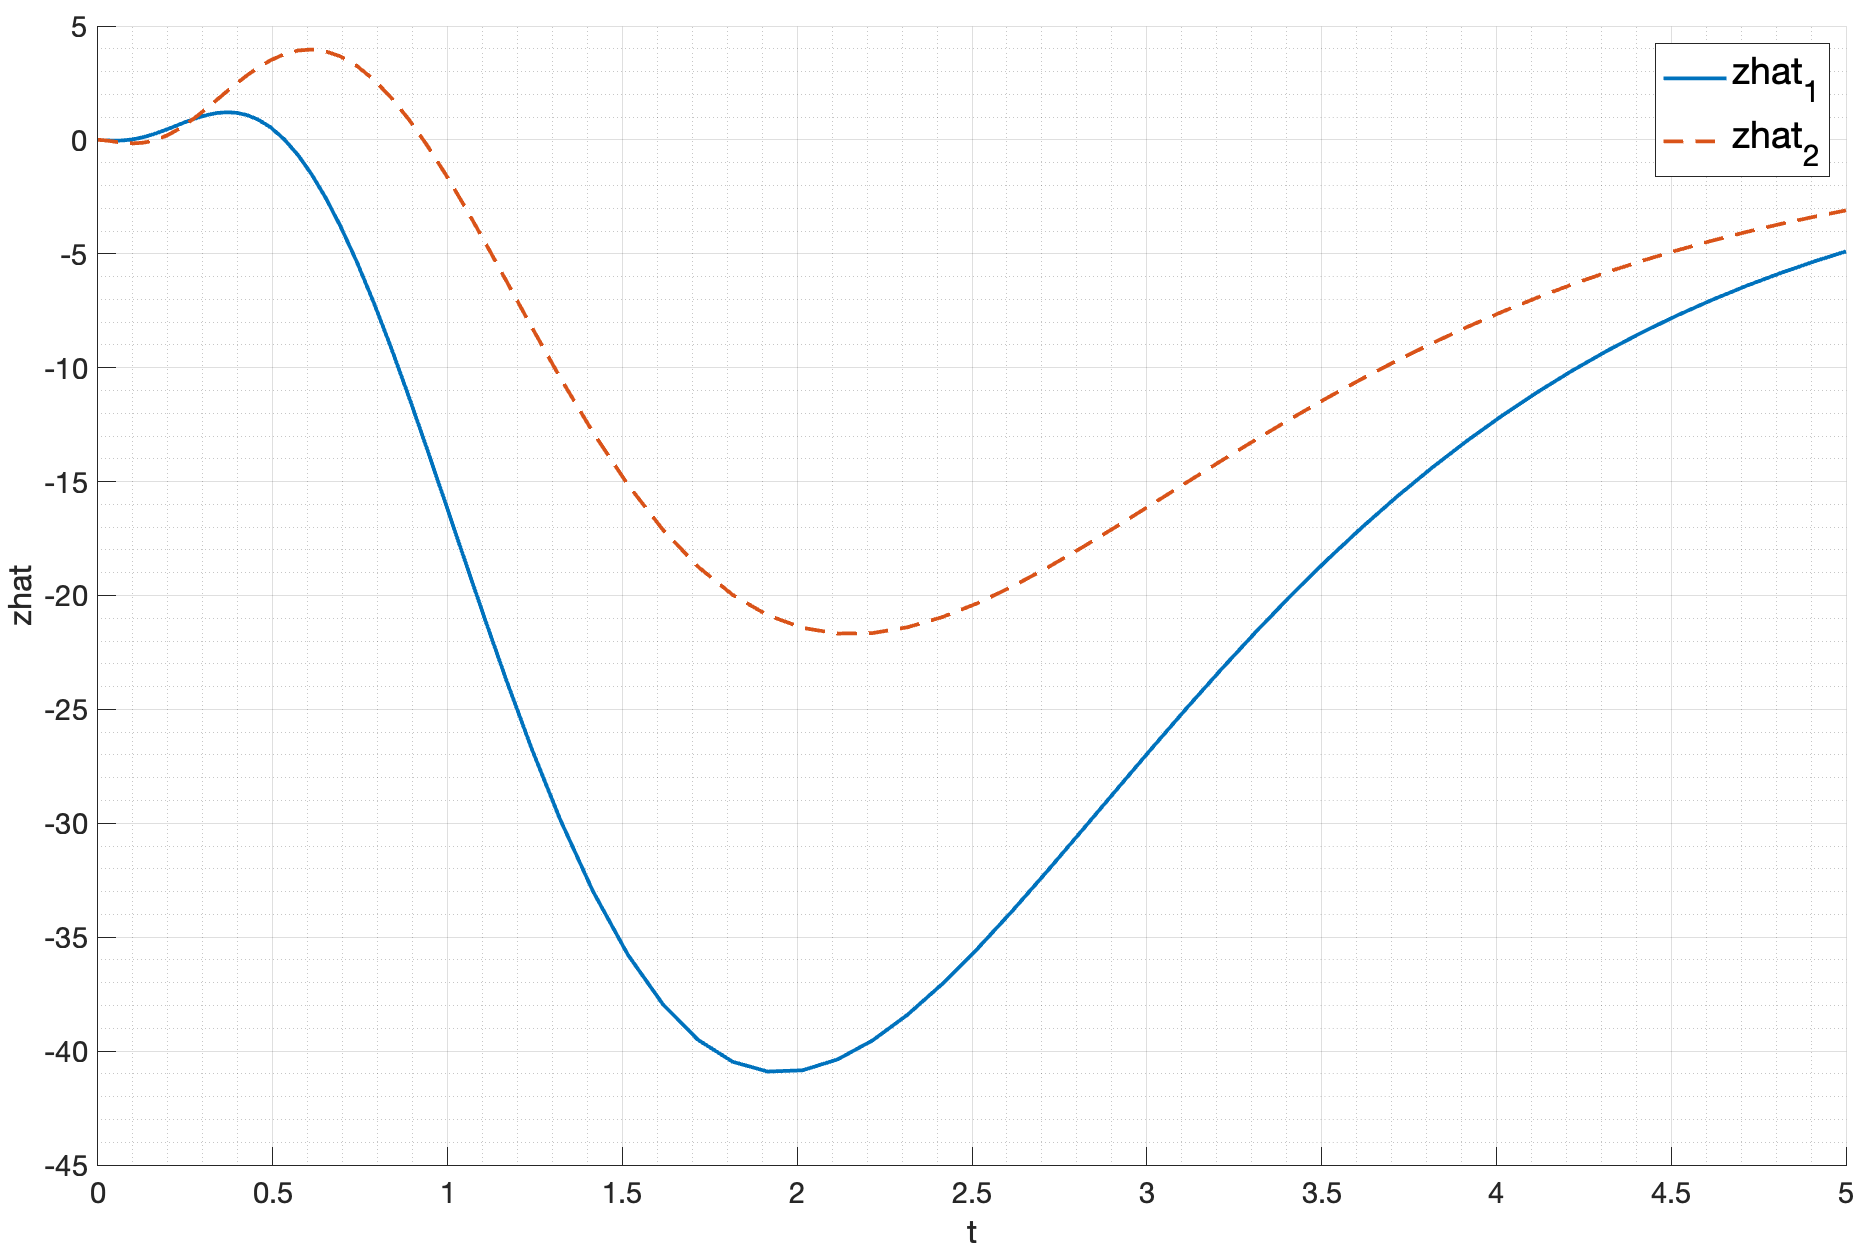
\includegraphics[width=\textwidth]{media/plots/task4_zhat_1.png}
    \caption{Вектор $\hat{z}$}
    \label{fig:task4_zhat_1}
\end{figure}

\FloatBarrier
\subsection{Выводы}
Видно, что оценка состояний $x_1$ и $x_2$ сходится к реальным значениям очень быстро, а 
состояния $x_3$ и $x_4$ сразу же имеют верные значения, так как они измеряются напрямую. 
Система управляется и наблюдается корректно.